\documentclass[12pt]{article}

\usepackage{fontspec}
\newfontfamily\handwriting{a-casual-handwritten-pen}[Path=../assets/fonts/,Extension=.ttf,Scale=1.5]
\newfontfamily\comic{Comic Neue}

\usepackage[utf8]{inputenc}
\usepackage{amsmath}
\usepackage{amssymb}
\usepackage{enumitem}
\usepackage{xcolor}
\usepackage{soul}
\usepackage{tikz}
\usepackage[most]{tcolorbox}
\usepackage{titlesec}
\usepackage{multicol}
\usepackage{environ}

\usetikzlibrary{fit, positioning, arrows.meta, decorations.pathreplacing}

% --- Custom Colors ---
\definecolor{primaryblue}{RGB}{42, 111, 151}
\definecolor{exbg}{RGB}{255, 240, 245}
\definecolor{rulebg}{RGB}{232, 245, 233}
\definecolor{highlight}{RGB}{255, 243, 176}
\definecolor{pinkanno}{RGB}{255, 105, 180}
\definecolor{purpleanno}{RGB}{147, 112, 219}
\definecolor{solutionbg}{RGB}{245, 245, 255}

% --- Header Styling ---
\titleformat{\section}{\color{primaryblue}\normalfont\Large\bfseries}{\thesection}{1em}{}
\titleformat{\subsection}{\color{primaryblue}\normalfont\large\bfseries}{\thesubsection}{1em}{}

% --- Friendly Boxes ---
% --- Auto-numbered Example Box ---
\newcounter{examplenum}

\newtcolorbox{friendlyexbox}[1]{
    colback=exbg,
    colframe=pinkanno!50,
    arc=5pt,
    title=\textbf{#1},
    coltitle=black,
    attach title to upper,
    after title={:\quad}
}

\newenvironment{friendlyex}{%
    \refstepcounter{examplenum}%
    \begin{friendlyexbox}{Example \theexamplenum}%
}{%
    \end{friendlyexbox}%
}

\newtcolorbox{friendlyrule}[1]{
    colback=rulebg,
    colframe=primaryblue!30,
    arc=5pt,
    fonttitle=\bfseries,
    title={#1},
    coltitle=primaryblue
}

\newcommand{\funhl}[1]{\sethlcolor{highlight}\hl{#1}}

% --- Show/Hide Solutions ---
\newif\ifshowsolutions

% Uncomment the next line to show solutions.
\showsolutionstrue

\newsavebox{\solutionmeasurebox}

\NewEnviron{solutionbox}{
\ifshowsolutions
\begin{tcolorbox}[
    colback=solutionbg,
    colframe=purpleanno!45,
    arc=5pt,
    title={Solution},
    coltitle=primaryblue,
    fonttitle=\bfseries
]
\BODY
\end{tcolorbox}
\else
\sbox{\solutionmeasurebox}{\begin{minipage}{\dimexpr\linewidth-10pt\relax}\BODY\end{minipage}}
\vspace{\dimexpr\ht\solutionmeasurebox+\dp\solutionmeasurebox+3em\relax}
\fi
}

\begin{document}
\handwriting

\begin{center}
    \Large\textbf{\color{primaryblue}Module 3 Lesson 1\\Introduction to Polynomial Functions} \\
    \vspace{0.2cm}
    \hrule
\end{center}

\section*{Objectives}

\begin{friendlyrule}{In this lesson, we will learn how to}
\begin{itemize}
    \item identify polynomial functions and their degree;
    \item determine end behavior using the leading-term test;
    \item find zeros of a polynomial and their multiplicity;
    \item classify zeros as cross or bounce points;
    \item find $x$- and $y$-intercepts of a polynomial function.
\end{itemize}
\end{friendlyrule}

\section*{1. Polynomial Functions}

\begin{friendlyrule}{Polynomial Function}
A function of the form

\[
f(x)=a_nx^n+a_{n-1}x^{n-1}+a_{n-2}x^{n-2}+\cdots+a_1x+a_0,\qquad a_n\neq 0,
\]

is a polynomial function.
\end{friendlyrule}

Examples:

\[
f(x)=2x^3-4x^2+5x-6,\qquad f(x)=-3x^5+7x-9,
\]

\[
y=4x^6-7x^2-6x^3-4x^4+5x-6,\qquad V=\frac43\pi r^3.
\]

\begin{itemize}
    \item The coefficients $a_n,a_{n-1},\ldots,a_2,a_1,a_0$ are \funhl{real numbers}. The powers $n,n-1,n-2,\ldots$ are \funhl{non-negative integers} (whole numbers).
    \item The \funhl{degree} of a polynomial function is the highest power of $x$ in the formula.
    \item The graph of a polynomial function is both \funhl{continuous} and \funhl{smooth}. Informally, a continuous function can be drawn without lifting the pencil from the paper, and a smooth function has no sharp corners or points.
\end{itemize}

\section*{2. Turning Points}

\begin{friendlyrule}{Turning Points}
A polynomial function of degree $n$ has \textbf{at most} $n-1$ hills or valleys (turning points).
\end{friendlyrule}

\textbf{Degree 2 (quadratic) --- 1 turning point}

\begin{center}
\begin{tikzpicture}[scale=0.4]
\begin{scope}
\draw[-{Latex}] (-3,0) -- (3,0);
\draw[-{Latex}] (0,-1.5) -- (0,3.5);
\draw[thick, domain=-2.2:2.2, samples=40, smooth] plot (\x, {0.5*\x*\x-1});
\end{scope}
\begin{scope}[shift={(8,0)}]
\draw[-{Latex}] (-3,0) -- (3,0);
\draw[-{Latex}] (0,-3.5) -- (0,1.5);
\draw[thick, domain=-2.2:2.2, samples=40, smooth] plot (\x, {-0.5*\x*\x+1});
\end{scope}
\end{tikzpicture}
\end{center}

\textbf{Degree 3 (cubic) --- at most 2 turning points}

\begin{center}
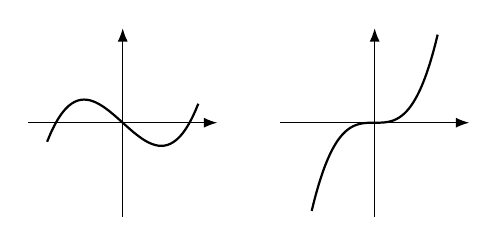
\begin{tikzpicture}[scale=0.4]
\begin{scope}
\draw[-{Latex}] (-3,0) -- (3,0);
\draw[-{Latex}] (0,-3) -- (0,3);
\draw[thick, domain=-2.4:2.4, samples=50, smooth] plot (\x, {0.2*\x*\x*\x-0.9*\x});
\end{scope}
\begin{scope}[shift={(8,0)}]
\draw[-{Latex}] (-3,0) -- (3,0);
\draw[-{Latex}] (0,-3) -- (0,3);
\draw[thick, domain=-2:2, samples=50, smooth] plot (\x, {0.35*\x*\x*\x});
\end{scope}
\end{tikzpicture}
\end{center}

\textbf{Degree 4 --- at most 3 turning points}

\begin{center}
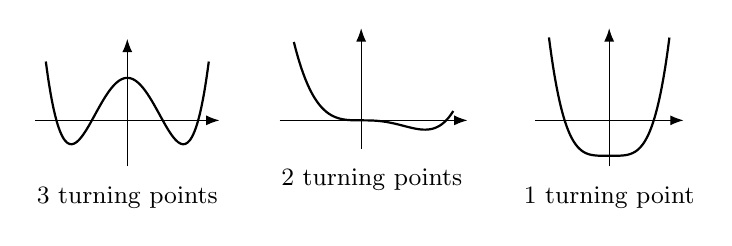
\begin{tikzpicture}[scale=0.45]
\begin{scope}
\draw[-{Latex}] (-2.6,0) -- (2.6,0);
\draw[-{Latex}] (0,-1.3) -- (0,2.3);
\draw[thick, domain=-2.3:2.3, samples=70, smooth] plot (\x, {0.3*(\x*\x*\x*\x-5*\x*\x+4)});
\node[below] at (0,-1.6) {\small 3 turning points};
\end{scope}
\begin{scope}[shift={(6.6,0)}]
\draw[-{Latex}] (-2.3,0) -- (3,0);
\draw[-{Latex}] (0,-0.8) -- (0,2.6);
\draw[thick, domain=-1.9:2.6, samples=70, smooth] plot (\x, {0.075*\x*\x*\x*\x-0.18*\x*\x*\x});
\node[below] at (0.3,-1.1) {\small 2 turning points};
\end{scope}
\begin{scope}[shift={(13.6,0)}]
\draw[-{Latex}] (-2.1,0) -- (2.1,0);
\draw[-{Latex}] (0,-1.3) -- (0,2.6);
\draw[thick, domain=-1.7:1.7, samples=60, smooth] plot (\x, {0.4*\x*\x*\x*\x-1});
\node[below] at (0,-1.6) {\small 1 turning point};
\end{scope}
\end{tikzpicture}
\end{center}

\section*{3. End Behavior (Leading-Term Test)}

The left-hand/right-hand end behavior is determined by (1) whether the degree is even or odd, and (2) the sign of the leading coefficient.

\textbf{Even Degree.} The ends shoot off in the \textbf{same} direction.
\begin{itemize}
    \item If the leading coefficient is positive, both ends go up.
    \item If the leading coefficient is negative, both ends go down.
\end{itemize}

\begin{center}
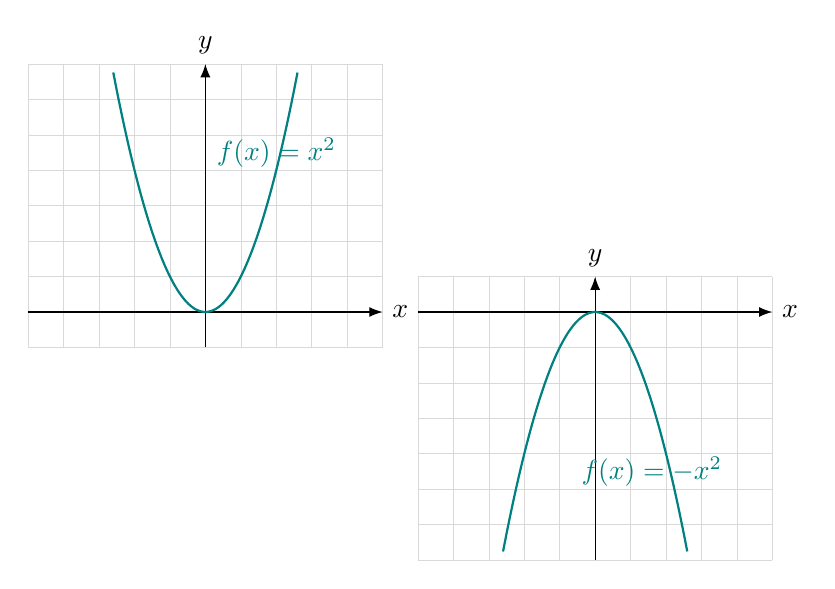
\begin{tikzpicture}[scale=0.45]
\begin{scope}
\draw[step=1, gray!30, very thin] (-5,-1) grid (5,7);
\draw[-{Latex}] (-5,0) -- (5,0) node[right] {$x$};
\draw[-{Latex}] (0,-1) -- (0,7) node[above] {$y$};
\draw[teal, thick, domain=-2.6:2.6, samples=50, smooth] plot (\x, {\x*\x});
\node[teal] at (2,4.5) {$f(x)=x^2$};
\end{scope}
\begin{scope}[shift={(11,0)}]
\draw[step=1, gray!30, very thin] (-5,-7) grid (5,1);
\draw[-{Latex}] (-5,0) -- (5,0) node[right] {$x$};
\draw[-{Latex}] (0,-7) -- (0,1) node[above] {$y$};
\draw[teal, thick, domain=-2.6:2.6, samples=50, smooth] plot (\x, {-\x*\x});
\node[teal] at (1.6,-4.5) {$f(x)=-x^2$};
\end{scope}
\end{tikzpicture}
\end{center}

\begin{center}
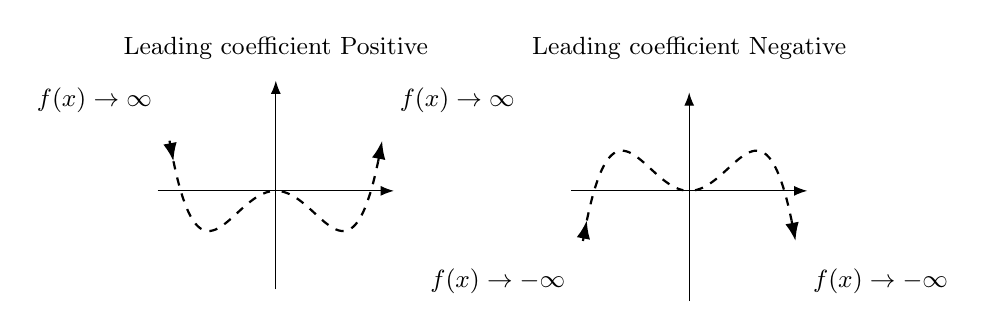
\begin{tikzpicture}[scale=0.5]
\begin{scope}
\node[above] at (0,3.1) {\small Leading coefficient Positive};
\draw[-{Latex}] (-3,0) -- (3,0);
\draw[-{Latex}] (0,-2.5) -- (0,2.8);
\draw[dashed, thick, domain=-2.6:-0.15, samples=40, smooth] plot (\x, {0.12*\x*\x*\x*\x-0.7*\x*\x});
\draw[thick, -{Latex}, domain=-2.7:-2.6, samples=2] plot (\x, {0.12*\x*\x*\x*\x-0.7*\x*\x});
\draw[dashed, thick, domain=0.15:2.6, samples=40, smooth] plot (\x, {0.12*\x*\x*\x*\x-0.7*\x*\x});
\draw[thick, -{Latex}, domain=2.6:2.7, samples=2] plot (\x, {0.12*\x*\x*\x*\x-0.7*\x*\x});
\node[anchor=east] at (-2.9,2.3) {\small $f(x)\to\infty$};
\node[anchor=west] at (2.9,2.3) {\small $f(x)\to\infty$};
\end{scope}
\begin{scope}[shift={(10.5,0)}]
\node[above] at (0,3.1) {\small Leading coefficient Negative};
\draw[-{Latex}] (-3,0) -- (3,0);
\draw[-{Latex}] (0,-2.8) -- (0,2.5);
\draw[dashed, thick, domain=-2.6:-0.15, samples=40, smooth] plot (\x, {-0.12*\x*\x*\x*\x+0.7*\x*\x});
\draw[thick, -{Latex}, domain=-2.7:-2.6, samples=2] plot (\x, {-0.12*\x*\x*\x*\x+0.7*\x*\x});
\draw[dashed, thick, domain=0.15:2.6, samples=40, smooth] plot (\x, {-0.12*\x*\x*\x*\x+0.7*\x*\x});
\draw[thick, -{Latex}, domain=2.6:2.7, samples=2] plot (\x, {-0.12*\x*\x*\x*\x+0.7*\x*\x});
\node[anchor=east] at (-2.9,-2.3) {\small $f(x)\to-\infty$};
\node[anchor=west] at (2.9,-2.3) {\small $f(x)\to-\infty$};
\end{scope}
\end{tikzpicture}
\end{center}

\textbf{Odd Degree.} The ends shoot off in \textbf{opposite} directions.
\begin{itemize}
    \item If the leading coefficient is positive, left down and right up.
    \item If the leading coefficient is negative, left up and right down.
\end{itemize}

\begin{center}
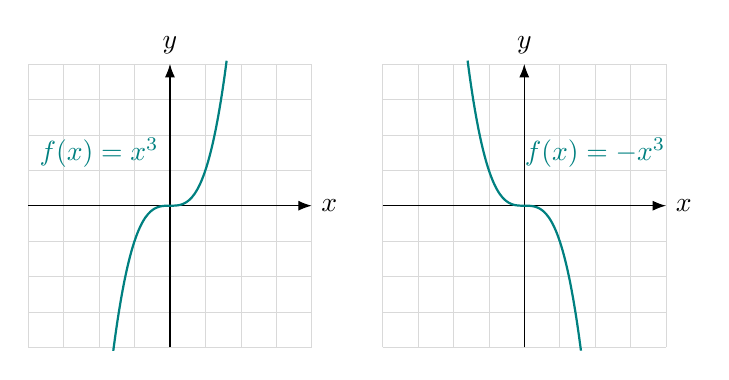
\begin{tikzpicture}[scale=0.45]
\begin{scope}
\draw[step=1, gray!30, very thin] (-4,-4) grid (4,4);
\draw[-{Latex}] (-4,0) -- (4,0) node[right] {$x$};
\draw[-{Latex}] (0,-4) -- (0,4) node[above] {$y$};
\draw[teal, thick, domain=-1.6:1.6, samples=50, smooth] plot (\x, {\x*\x*\x});
\node[teal] at (-2,1.5) {$f(x)=x^3$};
\end{scope}
\begin{scope}[shift={(10,0)}]
\draw[step=1, gray!30, very thin] (-4,-4) grid (4,4);
\draw[-{Latex}] (-4,0) -- (4,0) node[right] {$x$};
\draw[-{Latex}] (0,-4) -- (0,4) node[above] {$y$};
\draw[teal, thick, domain=-1.6:1.6, samples=50, smooth] plot (\x, {-\x*\x*\x});
\node[teal] at (2,1.5) {$f(x)=-x^3$};
\end{scope}
\end{tikzpicture}
\end{center}

\begin{center}
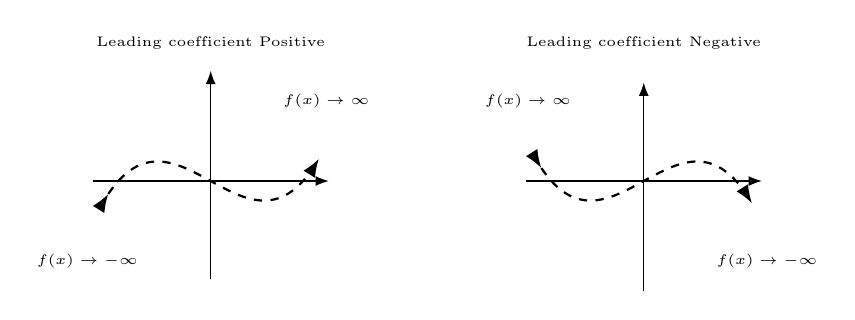
\begin{tikzpicture}[scale=0.5]
\begin{scope}
\node[above] at (0,3.1) {\tiny Leading coefficient Positive};
\draw[-{Latex}] (-3,0) -- (3,0);
\draw[-{Latex}] (0,-2.5) -- (0,2.8);
\draw[dashed, thick, domain=-2.6:2.6, samples=60, smooth] plot (\x, {0.1*\x*\x*\x-0.55*\x});
\draw[thick, -{Latex}, domain=2.6:2.75, samples=2] plot (\x, {0.1*\x*\x*\x-0.55*\x});
\draw[thick, -{Latex}, domain=-2.75:-2.6, samples=2] plot (\x, {0.1*\x*\x*\x-0.55*\x});
\node[anchor=south west] at (1.6,1.6) {\tiny $f(x)\to\infty$};
\node[anchor=north east] at (-1.6,-1.6) {\tiny $f(x)\to-\infty$};
\end{scope}
\begin{scope}[shift={(11,0)}]
\node[above] at (0,3.1) {\tiny Leading coefficient Negative};
\draw[-{Latex}] (-3,0) -- (3,0);
\draw[-{Latex}] (0,-2.8) -- (0,2.5);
\draw[dashed, thick, domain=-2.6:2.6, samples=60, smooth] plot (\x, {-0.1*\x*\x*\x+0.55*\x});
\draw[thick, -{Latex}, domain=2.6:2.75, samples=2] plot (\x, {-0.1*\x*\x*\x+0.55*\x});
\draw[thick, -{Latex}, domain=-2.75:-2.6, samples=2] plot (\x, {-0.1*\x*\x*\x+0.55*\x});
\node[anchor=north west] at (1.6,-1.6) {\tiny $f(x)\to-\infty$};
\node[anchor=south east] at (-1.6,1.6) {\tiny $f(x)\to\infty$};
\end{scope}
\end{tikzpicture}
\end{center}

\begin{friendlyex}{}
Determine the end behavior of each polynomial.

\begin{enumerate}[label=(\alph*)]
    \item $f(x)=3x^4-5x^2+1$
    \item $f(x)=-2x^5+3x^3-x$
    \item $f(x)=-4x^2+7x-1$
    \item $f(x)=6x^3-x^2+2$
    \item $f(x)=5x^6-2x+9$
\end{enumerate}
\end{friendlyex}

\begin{solutionbox}
\begin{enumerate}[label=(\alph*)]
    \item Degree $4$ (even), leading coefficient $3>0$: both ends go up ($f(x)\to\infty$ as $x\to\pm\infty$).
    \item Degree $5$ (odd), leading coefficient $-2<0$: left up, right down ($f(x)\to\infty$ as $x\to-\infty$, $f(x)\to-\infty$ as $x\to\infty$).
    \item Degree $2$ (even), leading coefficient $-4<0$: both ends go down ($f(x)\to-\infty$ as $x\to\pm\infty$).
    \item Degree $3$ (odd), leading coefficient $6>0$: left down, right up.
    \item Degree $6$ (even), leading coefficient $5>0$: both ends go up.
\end{enumerate}
\end{solutionbox}

\section*{4. Zeros and Multiplicity}

\begin{friendlyrule}{Zeros of a Polynomial}
A \funhl{zero} of a polynomial function $f$ is a value $c$ such that $f(c)=0$. If $(x-c)^m$ is a factor of $f(x)$ and $(x-c)^{m+1}$ is not, then $c$ is a zero of \funhl{multiplicity} $m$.
\end{friendlyrule}

\begin{friendlyex}{}
List the zeros of each polynomial and state their multiplicity.

\begin{enumerate}[label=(\alph*)]
    \item $f(x)=(x-2)^3(x+1)^2$
    \item $f(x)=x(x-4)(x+5)^4$
    \item $f(x)=-2(x-1)(x-3)^2(x+2)^5$
\end{enumerate}
\end{friendlyex}

\begin{solutionbox}
\begin{enumerate}[label=(\alph*)]
    \item $x=2$, multiplicity $3$ (odd); \quad $x=-1$, multiplicity $2$ (even).
    \item $x=0$, multiplicity $1$ (odd); \\
    $x=4$, multiplicity $1$ (odd); \\
    $x=-5$, multiplicity $4$ (even).
    \item $x=1$, multiplicity $1$ (odd); \\
    $x=3$, multiplicity $2$ (even); \\
    $x=-2$, multiplicity $5$ (odd).
\end{enumerate}
\end{solutionbox}

\section*{5. Cross vs.\ Bounce Points}

\begin{friendlyrule}{Behavior at a Zero}
\begin{itemize}
    \item If the multiplicity $m$ is \funhl{odd}, the graph \textbf{crosses} the $x$-axis at $c$.
    \item If the multiplicity $m$ is \funhl{even}, the graph \textbf{touches} the $x$-axis and \textbf{bounces back} (turns around) at $c$.
\end{itemize}
\end{friendlyrule}

\begin{center}
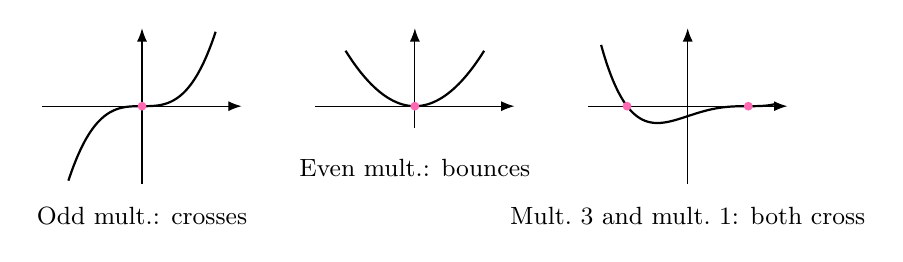
\begin{tikzpicture}[scale=0.55]
\begin{scope}
\draw[-{Latex}] (-2.3,0) -- (2.3,0);
\draw[-{Latex}] (0,-1.8) -- (0,1.8);
\draw[thick, domain=-1.7:1.7, samples=50, smooth] plot (\x, {0.35*\x*\x*\x});
\filldraw[pinkanno] (0,0) circle (2.5pt);
\node[below] at (0,-2.1) {\small Odd mult.: crosses};
\end{scope}
\begin{scope}[shift={(6.3,0)}]
\draw[-{Latex}] (-2.3,0) -- (2.3,0);
\draw[-{Latex}] (0,-0.5) -- (0,1.8);
\draw[thick, domain=-1.6:1.6, samples=50, smooth] plot (\x, {0.5*\x*\x});
\filldraw[pinkanno] (0,0) circle (2.5pt);
\node[below] at (0,-1) {\small Even mult.: bounces};
\end{scope}
\begin{scope}[shift={(12.6,0)}]
\draw[-{Latex}] (-2.3,0) -- (2.3,0);
\draw[-{Latex}] (0,-1.8) -- (0,1.8);
\draw[thick, domain=-2:2, samples=60, smooth] plot (\x, {0.06*(\x-1.4)*(\x-1.4)*(\x-1.4)*(\x+1.4)});
\filldraw[pinkanno] (1.4,0) circle (2.5pt);
\filldraw[pinkanno] (-1.4,0) circle (2.5pt);
\node[below] at (0,-2.1) {\small Mult.\ 3 and mult.\ 1: both cross};
\end{scope}
\end{tikzpicture}
\end{center}

\begin{friendlyex}{}
Find the zeros of each polynomial and classify each as a cross point or bounce point.

\begin{enumerate}[label=(\alph*)]
    \item $f(x)=x^4+4x^3+3x^2$
    \item $f(x)=x^3-5x^2-x+5$
\end{enumerate}
\end{friendlyex}

\begin{solutionbox}
\textbf{(a)} Factor out the GCF, then factor the remaining trinomial:
\[
f(x)=x^2(x^2+4x+3)=x^2(x+1)(x+3).
\]
Zeros: $x=0$ (mult.\ $2$, bounce), $x=-1$ (mult.\ $1$, cross), $x=-3$ (mult.\ $1$, cross).

\textbf{(b)} Factor by grouping:
\[
f(x)=x^2(x-5)-1(x-5)=(x-5)(x^2-1)=(x-5)(x-1)(x+1).
\]
Zeros: $x=5,\ x=1,\ x=-1$, each multiplicity $1$ (all cross points).
\end{solutionbox}

\section*{6. Intercepts}

\begin{friendlyrule}{Finding Intercepts}
\begin{itemize}
    \item $y$-intercept: evaluate $f(0)$.
    \item $x$-intercepts: solve $f(x)=0$ (these are the zeros of $f$).
\end{itemize}
\end{friendlyrule}

\begin{friendlyex}{}
Find the $x$- and $y$-intercepts of $f(x)=(x-2)(x+1)(x+4)$.
\end{friendlyex}

\begin{solutionbox}
$x$-intercepts (zeros): $x=2,\ x=-1,\ x=-4$, i.e.\ $(2,0),\ (-1,0),\ (-4,0)$.

$y$-intercept: $f(0)=(0-2)(0+1)(0+4)=(-2)(1)(4)=-8$, i.e.\ $(0,-8)$.
\end{solutionbox}

\section*{7. Reasoning About Degree}

\begin{friendlyex}{}
A polynomial's graph has exactly $2$ turning points and both ends rise. What is the smallest possible degree, and is the leading coefficient positive or negative?
\end{friendlyex}

\begin{solutionbox}
A degree-$n$ polynomial has at most $n-1$ turning points, so $2$ turning points requires degree at least $3$. Since both ends rise, the degree must be \textbf{even}, so the smallest possible degree is $\boxed{4}$. Both ends rising means the leading coefficient is \textbf{positive}.
\end{solutionbox}

\begin{friendlyex}{}
A polynomial's graph crosses the $x$-axis at $x=-3,0,2$ and has $y$-intercept $0$. Both ends of the graph fall. What is the smallest possible degree?
\end{friendlyex}

\begin{solutionbox}
Three distinct crossing zeros require at least degree $3$ (odd). But both ends falling means the same direction on both sides, which requires an \textbf{even} degree. The smallest even degree that can still produce $3$ sign changes (crossings) is $\boxed{4}$ --- one of the zeros would need even multiplicity, e.g.\ $f(x)=-(x+3)(x)(x-2)^2$, or another zero is repeated so total multiplicity is $4$.
\end{solutionbox}

\begin{friendlyex}{}
The graph of a polynomial touches the $x$-axis at $x=1$ without crossing, and crosses at $x=-2$. What is the smallest possible degree?
\end{friendlyex}

\begin{solutionbox}
Touching (bounce) at $x=1$ requires even multiplicity, smallest is $2$. Crossing at $x=-2$ requires odd multiplicity, smallest is $1$. Total smallest degree: $2+1=\boxed{3}$.
\end{solutionbox}

\section*{Summary}

\begin{friendlyrule}{Key Ideas}
\begin{itemize}
    \item A polynomial function has the form $a_nx^n+\cdots+a_1x+a_0$; its degree is the highest power of $x$, and its graph is always continuous and smooth.
    \item A degree-$n$ polynomial has \textbf{at most} $n-1$ turning points.
    \item End behavior is determined by the degree's parity and the leading coefficient's sign: even degree $\to$ both ends the same direction; odd degree $\to$ opposite directions; positive leading coefficient $\to$ right end up; negative $\to$ right end down.
    \item If $(x-c)^m$ is a factor of $f(x)$, then $c$ is a zero of multiplicity $m$: \textbf{odd} multiplicity $\to$ the graph \textbf{crosses} the $x$-axis; \textbf{even} multiplicity $\to$ the graph \textbf{bounces}.
    \item The $y$-intercept is $f(0)$; the $x$-intercepts are the zeros of $f$.
\end{itemize}
\end{friendlyrule}

\end{document}
